\mychapter{2}{Background}

The first step that will be taken to investigate how the parameters could be automated will be to first review the background of backflow, as well as the methods used to stabilise it. An important equation will also be derived that will be the basis of the stability criterion detailed further in the next chapter.\\

\autoref{fig:instab} shows graphically that the presence of backflow at open boundaries, boundaries where a natural boundary condition is prescribed, may cause the numerical simulation to become unstable.
\begin{figure}[t]
\centering
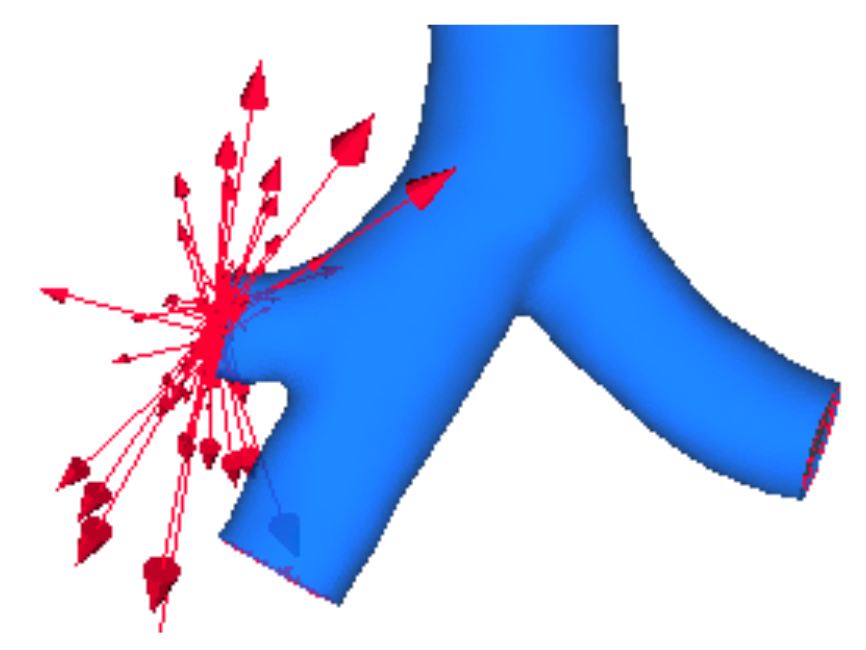
\includegraphics[width=5cm]{media/instability.PNG}
\caption{Example of numerical instability due to backflow\label{fig:instab}}
\end{figure}
This instability is consistent in that in the presence of backflow there is a lack of general well-posedness results for the incompressible Navier-Stokes equations \cite[429--430]{alfioquarteroni2014}: \begin{align}\label{eq:NSeq}\begin{split}
 \rho\partial_t\bmu + \rho(\bmu - \textbf{w})\cdot\nabla\bmu - 2\mu\nabla\cdot\bm{\varepsilon}(\bmu) + \nabla p &= 0\quad\text{on}~\Omega \\ \nabla\cdot\bmu &= 0\quad\text{on}~\Omega \\
 \bmu &= \bm{\phi}\quad\text{on}~\Gamma_D\\
 2\mu\bm{\varepsilon}(\bmu)\bmn - p\bmn &= \bm{\psi}\quad\text{on}~\Gamma_N
 \end{split}\end{align}
 where \mathm{\rho} is the density, \bmu~is the background flow of the fluid, \textbf{w} is the flow of the domain, \mathm{\mu} is the viscosity, \mathm{\stresstens = \frac{1}{2}\qty(\nabla\bmu + \nabla\bmu^\text{T})} is the strain rate tensor and \mathm{p} is the pressure. \mathm{\Omega \subset \mathds{R}^d}(with \mathm{d} = 2,3) is the entire domain, \mathm{\Gamma_{D}} is the boundary with the Dirichlet boundary condition, \mathm{\Gamma_{N}} is the boundary with the Neumann boundary condition and so \mathm{\partial\Omega = \Gamma_{D}\bigcup\Gamma_{N}}. 
 
 \section{Energy Estimate}
 To see the instability issue, \autoref{eq:NSeq} can be rewritten while also assuming that \mathm{\phi} and \mathm{\psi} are \mathm{\bm{0}}. We take the first equation of \eqref{eq:NSeq} and dot each term with the flow, \bmu, and following that integrate over the entire domain:
 \begin{equation}\label{eq:NSenergy1}
     \fint\rho\partial_t\bmu \cdot \bmu + \fint\rho\bmu\cdot\nabla\bmu \cdot \bmu - 2\mu\fint\nabla\cdot\bm{\varepsilon}(\bmu) \cdot \bmu + \fint\nabla p \cdot \bmu = 0.
 \end{equation}
 
 \noindent Noting that \mathm{\partial_{t}\norm{\bmu}^2 = \partial_{t}\qty(\bmu\cdot\bmu) = \partial_{t}\bmu\cdot\bmu + \bmu\cdot\partial_{t}\bmu = 2\qty(\partial_{t}\bmu\cdot\bmu)} and similarly that \mathm{\nabla\norm{\bmu}^2 = 2\qty(\nabla\bmu\cdot\bmu)}, the first and second terms of \eqref{eq:NSenergy1} can be rewritten, resulting in:
 
 \begin{equation}\label{eq:NSenergy2}
  \frac{\rho}{2}\partial_{t}\fint\norm{\bmu}^2 + \frac{\rho}{2}\fint\bmu\cdot\nabla\norm{\bmu}^2 - 2\mu\fint\nabla\cdot\bm{\varepsilon}(\bmu) \cdot \bmu + \fint\nabla p \cdot \bmu = 0
 \end{equation}
 To proceed, the third and fourth term of \eqref{eq:NSenergy2} will need to be rewritten. First consider the integrand of the third term of \eqref{eq:NSenergy2}:
 \begin{align*}
     \qty(\nabla\cdot\stresstens)\cdot\bmu &= \sum_j \qty(\nabla\cdot\stresstens)_{j}\bmu_{j} \tag*{(Writing out definition of dot product)}\\
        \intertext{We can also use the fact that for any matrix \mathm{A}, the \mathm{j}-th element of the divergence of \mathm{A} is the divergence of the \mathm{j}-th column of \mathm{A}. Thus:}
        &= \sum_j \qty(\nabla\cdot\stresstens^{j})\bmu_{j} \tag*{(Where \mathm{\stresstens^j} is the \mathm{j}-th column of \mathm{\stresstens})}\\
        &= \sum_j \sum_i \qty(\pdv{\stresstens^j_i}{x_i})\bmu_j \tag*{(Expanding def. of divergence)}\\
        &= \sum_j \sum_i \qty(\pdv{\stresstens_{i,j}}{x_i})\bmu_j \tag*{(Rewriting the index notation)}\\
        \intertext{Here note that by the product rule: \mathm{\pdv{}{x_i}\qty(\stresstens_{i,j}\bmu) = \pdv{}{x_i}\qty(\stresstens_{i,j})\bmu + \pdv{}{x_i}\qty(\bmu)\stresstens_{i,j}}. Substituting this into the equation:}
        &= \sum_j \sum_i \qty(\qty(\pdv{}{x_i}\qty(\stresstens_{i,j}\bmu_j)) - \qty(\pdv{\bmu_j}{x_i})\stresstens_{i,j})\\
        &= \sum_j \sum_i \qty(\pdv{}{x_i}\qty(\stresstens_{i,j}\bmu_j)) - \sum_j \sum_i \qty(\pdv{\bmu_j}{x_i})\stresstens_{i,j} \\
\end{align*}
The first term is clearly the divergence of \mathm{\stresstens\bmu} however the second term is not immediately obvious. Consider however the following matrix multiplication of \mathm{\stresstens\nabla\bmu}:\\
\[
\begin{bmatrix}
\sum_{j}\stresstens_{1,j}\nabla\bmu_{j,1} & \sum_{j}\stresstens_{1,j}\nabla\bmu_{j,2} & \hdots \\
\sum_{j}\stresstens_{2,j}\nabla\bmu_{j,1} & \sum_{j}\stresstens_{2,j}\nabla\bmu_{j,2} & \hdots \\
\vdots  & \vdots  & \ddots
\end{bmatrix}
\]
from which we can see that second term is actually the trace of the above matrix, and thus:
\begin{equation*}
\qty(\nabla\cdot\stresstens)\cdot\bmu = \nabla\cdot\qty(\stresstens\bmu) - \stresstens\bm{:}\nabla\bmu
\end{equation*}
where for matrices \mathm{A} and \mathm{B} the double dot product \mathm{A\bm{:}B = \text{trace}\qty(AB)}. Taking a domain integral across all terms yields:
\begin{align}
    \fint\qty(\nabla\cdot\stresstens)\cdot\bmu &= \fint\nabla\cdot\qty(\stresstens\bmu) - \fint\stresstens\bm{:}\nabla\bmu \notag\\
            &= \int\limits_{\partial\Omega}\qty(\stresstens\bmu)\cdot\bmn - \fint\stresstens\bm{:}\nabla\bmu \tag*{(using divergence theorem)}\\
            \intertext{Finally using that due to \mathm{\stresstens} being symmetric, one can write \mathm{\qty(\stresstens\bmu)\cdot\bmn = \inner{\stresstens\bmu}{\bmn} = \inner{\bmu}{\stresstens^T\bmn} = \inner{\bmu}{\stresstens\bmn} = \qty(\stresstens\bmn)\cdot\bmu} and so:}
            &= \int\limits_{\partial\Omega}\qty(\stresstens\bmn)\cdot\bmu - \fint\stresstens\bm{:}\nabla\bmu \label{eq:stresstensByParts}
\end{align}
The third term of \eqref{eq:NSenergy2} has now been rewritten, and similarly for the fourth term note that \mathm{\nabla\cdot\qty(p\bmu) = p\nabla\cdot\bmu + \qty(\nabla p)\cdot\bmu} therefore:
\begin{align}
    \fint\qty(\nabla p)\cdot\bmu &= \fint\nabla\cdot\qty(p\bmu) - \fint  p\nabla\cdot\bmu \notag\\
                    &= \int\limits_{\partial\Omega}\qty(p\bmu)\cdot\bmn - \fint  p\nabla\cdot\bmu \tag*{(using divergence theorem)}\\
                    &= \int\limits_{\partial\Omega}\qty(p\bmn)\cdot\bmu - \fint  p\nabla\cdot\bmu\label{eq:pressureByParts}
\end{align}
 We can now substitute \eqref{eq:stresstensByParts} and \eqref{eq:pressureByParts} into \eqref{eq:NSenergy2}:
 \begin{multline}\label{eq:NSenergy3}
     \frac{\rho}{2}\partial_{t}\fint\norm{\bmu}^2 + \frac{\rho}{2}\fint\bmu\cdot\nabla\norm{\bmu}^2 + 2\mu\fint\bm{\varepsilon}(\bmu) \bm{:} \nabla\bmu\\ - \fint p\nabla\cdot\bmu - \int\limits_{\partial\Omega}\qty(2\mu\bm{\varepsilon}(\bmu) - p\mathbf{I})\bmn \cdot \bmu = 0
 \end{multline}
 However \mathm{\nabla\cdot\bmu = 0} from \eqref{eq:NSeq}, and thus \mathm{\int_{\Omega} p\nabla\cdot\bmu = 0}. It was assumed that \mathm{\bmu = \bm{0}} on \mathm{\Gamma_D} thus the boundary integral in \eqref{eq:NSenergy3} becomes an integral only over \mathm{\Gamma_N}, however from the other boundary condition, it was assumed that \mathm{\psi = \bm{0}} and so the entire final term of \eqref{eq:NSenergy3} is 0. Finally noting that \mathm{\bm{\varepsilon}(\bmu) \bm{:} \nabla\bmu = \bm{\varepsilon}(\bmu) \bm{:} \bm{\varepsilon}(\bmu)} results in:
 
 \begin{equation}\label{eq:NSenergy4}
     \frac{\rho}{2}\partial_{t}\fint\norm{\bmu}^2 + \frac{\rho}{2}\fint\bmu\cdot\nabla\norm{\bmu}^2 + 2\mu\fint\norm{\bm{\varepsilon}(\bmu)}^2  = 0
 \end{equation}
 Applying integration by parts to the second term of \eqref{eq:NSenergy4} yields:
 
  \begin{equation}\label{eq:NSenergy5}
     \frac{\rho}{2}\partial_{t}\fint\norm{\bmu}^2 - \frac{\rho}{2}\fint\nabla\cdot\bmu\norm{\bmu}^2 +
     \frac{\rho}{2}\int\limits_{\partial\Omega}\bmu\cdot\bmn\norm{\bmu}^2 +
     2\mu\fint\norm{\bm{\varepsilon}(\bmu)}^2  = 0
 \end{equation}
 After reordering terms and again noting that \mathm{\nabla\cdot\bmu = 0} and that \bmu~is 0 on \mathm{\Gamma_D} gives us the desired result:
 
\begin{equation}\label{NSeqENergy}
\partial_t\frac{\rho}{2}\fint\norm{\bmu}^2 = -2\mu\fint\norm{\bm{\varepsilon}(\bmu)}^2 - \underbrace{\frac{\rho}{2}\bint\bmu\cdot\bmn\norm{\bmu}^2}_{(\text{\large \textasteriskcentered})}
\end{equation}
The term ({\large \textasteriskcentered}) has been particularly highlighted because it is this term which causes the instability when trying to solve \autoref{eq:NSeq} with open boundaries. It is this term that must be countered in order to obtain stable solutions. Furtheremore \eqref{NSeqENergy} is the main result of this chapter, and will be used at the basis of the stability criterion derived in the next chapter.\\
\\
\autoref{eq:NSeq} will however not be solved analytically, as in general this is not possible for the Navier-Stokes equations, but rather wil be solved numerically using for instance a finite element method. To this end, a weak formulation of \eqref{eq:NSeq} \includecomment{Review the spaces for u and p} is required. The problem then becomes to find \bmu~\mathm{\in\mathbf{V}}and \mathm{p}~\mathm{\in\mathbf{Q}} such that \cite[433]{alfioquarteroni2014}:
\begin{align}\label{eq:NSweak}
\begin{split}
    \rho\inner{\partial_t\bmu}{\bmv}_{\Omega} ~+~
    \mu\inner{\nabla\bmu}{\nabla\bmv}_{\Omega} ~+~\\
    \rho\inner{\qty(\bmu\cdot\nabla)\bmu}{\bmv}_{\Omega} ~-~
    \rho\inner{p}{\nabla\cdot\bmv}_{\Omega} ~&=~ 0 \qquad \forall~\bmv~\in~\mathbf{V}\\
    \inner{\nabla\cdot\bmu}{\textbf{q}}_{\Omega} ~&=~ 0 \qquad \forall~\textbf{q}~\in~\mathbf{Q}
\end{split}
\end{align}
where the usual inner product \mathm{\inner{\bm{s}}{\bm{r}}_{\chi} = \int_{\chi} \bm{s} \cdot \bm{r}} and the following sub-spaces of the Lebesgue function space \mathm{L^2\qty(\Omega)} of square-integrable functions on \mathm{\Omega} are used:
\begin{align*}
\mathbf{Q} &:= \begin{cases}L^2_0\qty(\Omega) = \qty{\bmv \in L^2\qty(\Omega) : \inner{\bmv}{1}=0} & \Gamma_N = \emptyset,\\
L^2\qty(\Omega) & \Gamma_N \neq \emptyset,\end{cases}\\
H^1\qty(\Omega) &= \qty{\bmv \in L^2\qty(\Omega), \partial_i \bmv \in L^2\qty(\Omega), 1\leq i \leq d},\\
\mathbf{V} &:= H^1_0\qty(\Gamma_D;\Omega) = \qty{\bmv \in H^1\qty(\Omega), \bmv_{|\Gamma_D} = 0}.\\
\end{align*}
% Using the weak form, a discretised \todo{add discretised form}
The weak form as defined in \eqref{eq:NSweak} inherits the instability from the continuous case, and so when trying to solve the Navier-Stokes equations using a numerical method, this instability also needs to be taken into account and this is done by modifying and adding terms to the equations in order to counteract the instability.

\section{Backflow Stabilisation}
Up to date, several proposals to overcome this issue of backflow instability have appeared in literature, mainly consisting in modifying the natural boundary conditions in order to enhance the overall stability \cite{bertoglio2017}. Two main methods, Velocity Penalisation and Tangential Derivative Penalisation will be considered as well as a variant of the Tangential Derivative Penalisation. 
\subsubsection{Velocity Penalisation}
The Velocity Penalisation method relies on counteracting the energy of ({\large \textasteriskcentered}) by modifying the natural boundary condition where backflow occurs with \cite{Bruneau1994}:
\begin{align}\label{eq:VeloPenal}
    2\mu\stresstens\bmn - p{\bmn} ~{ + ~\beta\frac{\rho}{2}\abs{\bmu\cdot \bmn}_{-}\bmu} = \bm{\psi}, \qquad \beta \leq 1
\end{align}
where \mbeta~is an adjustable parameter currently chosen at the beginning of computation, and \mathm{\abs{\bmu\cdot \bmn}_{-} = \frac{\abs{\bmu\cdot \bmn} - \bmu\cdot \bmn}{2}}~ is the negative part of \mathm{\bmu\cdot\bmn}. Furthermore, this would result in the addition of the following term to \autoref{eq:NSweak}:
\begin{equation}\label{eq:stabVeloPen}
    S_{Vel} = \beta\frac{\rho}{2}\bint\abs{\bmu\cdot\bmn}_{-}\bmu\cdot\bmv
\end{equation}
This adjustment however has the issue that accuracy is affected by the extra term, especially since the outflow is perturbed by counteracting the backflow, though it has been proven that a value of \mbeta~=~1 will guarantee stability of the solution \cite{Bruneau1996}.
\subsubsection{Tangential Derivative Penalisation}
The Tangential Derivative Penalisation method plays on the idea of rather stabilising the local derivative of where the backflow occurs by the addition of either of the following terms to \autoref{eq:NSweak} \cite[Slide 21]{bertoglioLec12}:% adjusting \autoref{NSeqENergy} with:  
\begin{align}
S_{TangMax} &= \gamma U_b h^2 \frac{\rho}{2} \sum_{j=1}^{d-1}\bint \qty(t_j^{T}\nabla\bmu \cdot t_j^{T}\nabla\bmv) \qquad U_b = \max \abs{\bmu \cdot \bmn}_-\label{eq:stabTangPenMax}\\
    S_{Tang} &= \gamma h^2 \frac{\rho}{2} \sum_{j=1}^{d-1}\bint\abs{\bmu \cdot \bmn}_{-}\qty(t_j^{T}\nabla\bmu \cdot t_j^{T}\nabla\bmv)\label{eq:stabTangPen}
\end{align}
where \mgamma~is the stabilisation parameter and the \mathm{t_{j}}'s are the tangential directions. \mathm{S_{TangMax}}, referred hereafter as Tangential Penalisation Max method, guarantees stability for \mathm{h^{2}\gamma=C^{2}_{\Gamma_{N}^{b}}} where \mathm{C_{\Gamma_{N}^{b}}} is the Poincar\'e Constant of \mathm{\Gamma_{N}^{b} := \qty{\bm{x}\in\Gamma_{N} : \bmu\cdot\bmn<0}} \cite{bertoglio2016}. \mathm{S_{Tang}}, hereafter called Tangential Penalisation method, is a proposed simplification of \eqref{eq:stabTangPenMax} where there has not been a proven value of \mgamma~which guarantees stability however it has been shown to work well numerically \cite[Slide 25]{bertoglioLec12}\cite{bertoglio2014}. The Tangential Penalisation method appears to produce more accurate solutions as compared to the Velocity Penalisation method as seen in \autoref{fig:velocompare} and \autoref{fig:presscompare}, furthermore \autoref{fig:flowcompare} shows how both methods compare when simulating the velocity profile on real geometry \cite{bertoglio2017}.
% \begin{align}\label{eq:TangPenal}
% \partial_t\frac{\rho}{2}\fint\norm{\bmu}^2 = -2\mu\fint\norm{\bm{\varepsilon}(\bmu)}^2 - \frac{\rho}{2}\bint\bmu\cdot\bmn\norm{\bmu}^2 ~{\color{red}- ~\frac{\rho}{2}\bint\gamma\norm{{\bf t^{\text{T}}\nabla}\bmu}^2}
% \end{align}


In summary, The following stabilised weak formulation of \eqref{eq:NSeq} is defined:
\begin{align}\label{eq:NSweakstab}
\begin{split}
    \rho\inner{\partial_t\bmu}{\bmv}_{\Omega} ~+~
    \mu\inner{\nabla\bmu}{\nabla\bmv}_{\Omega} ~+~
    \rho\inner{\qty(\bmu\cdot\nabla)\bmu}{\bmv}_{\Omega} ~&-~\\
    \rho\inner{p}{\nabla\cdot\bmv}_{\Omega} ~+~ S ~&=~ 0 \qquad \forall~\bmv~\in~\mathbf{V}\\
    \inner{\nabla\cdot\bmu}{\textbf{q}}_{\Omega} ~&=~ 0 \qquad \forall~\textbf{q}~\in~\mathbf{Q}
\end{split}
\end{align}
where \mathm{S} is one of the before mentioned stabilisation methods, \mathm{S_{Vel}}, \mathm{S_{TangMax}} and \mathm{S_{Tang}}


\begin{figure}[t]
\centering
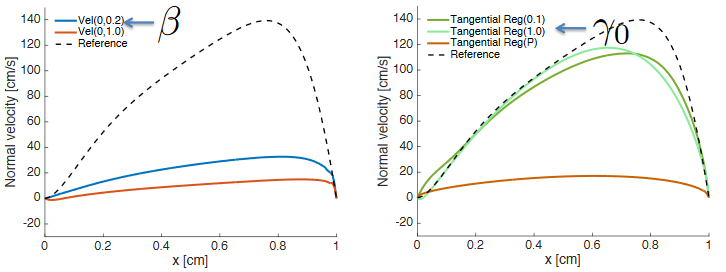
\includegraphics[width=\textwidth]{media/compare.PNG}
\caption{Comparison of methods for a velocity profile\label{fig:velocompare}}
\end{figure}
\begin{figure}[t]
\centering
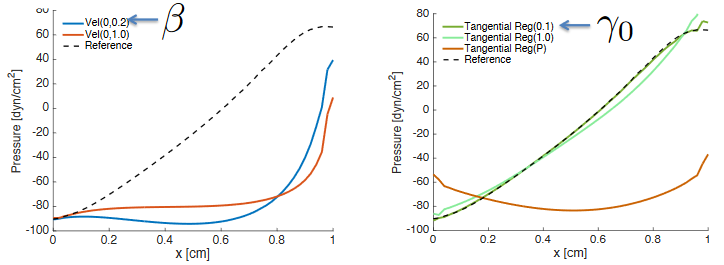
\includegraphics[width=\textwidth]{media/presscompare.PNG}
\caption{Comparison of methods for a pressure profile\label{fig:presscompare}}
\end{figure}
\begin{figure}[t]
\centering
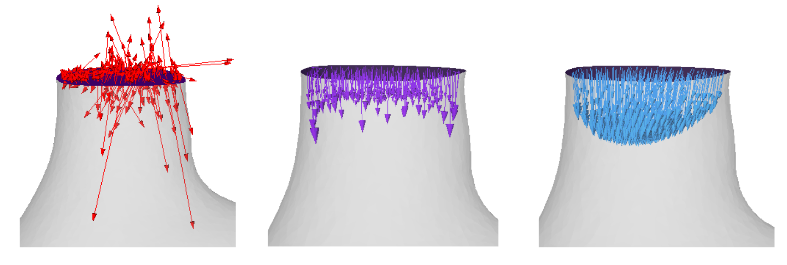
\includegraphics[width=\textwidth]{media/flowcomp.PNG}
\caption{Comparison of methods on a real geometry\label{fig:flowcompare}}
\end{figure}